% PP-Article.tex for AEA last revised 22 June 2011
\documentclass[twocolumn, a4paper]{article}

%\usepackage{amsmath}
\usepackage[dutch]{babel}
\usepackage{subcaption}
\usepackage[width=.8\textwidth]{caption}
\usepackage{float}
\usepackage{booktabs}
\usepackage{multicol}
\usepackage{minted}
% If you have trouble with the mathtime package please see our technical support 
% document at: http://www.aeaweb.org/templates/technical_support.pdf
% You may remove the mathtime package if you can't get it working but your page
% count may be inaccurate as a result.
% \usepackage[cmbold]{mathtime}
\usepackage{xargs}                      % Use more than one optional parameter in a new commands
\usepackage[pdftex,dvipsnames]{xcolor}  % Coloured text etc.
% 
\usepackage{pdfpages}
\usepackage[colorinlistoftodos,prependcaption,textsize=tiny]{todonotes}
\newcommandx{\unsure}[2][1=]{\todo[linecolor=red,backgroundcolor=red!25,bordercolor=red,#1]{#2}}
\setlength{\marginparwidth}{2cm}
% Note: you may use either harvard or natbib (but not both) to provide a wider
% variety of citation commands than latex supports natively. See below.

% Uncomment the next line to use the natbib package with bibtex 
%\usepackage{natbib}
\usepackage{titlesec}

%\titlespacing*\section{0pt}{12pt plus 4pt minus 2pt}{0pt plus 2pt minus 2pt}
%\titlespacing*\subsection{0pt}{12pt plus 4pt minus 2pt}{0pt plus 2pt minus 2pt}
%\titlespacing*\subsubsection{0pt}{12pt plus 4pt minus 2pt}{0pt plus 2pt minus 2pt}

% Uncomment the next line to use the harvard package with bibtex
%\usepackage[abbr]{harvard}

% This command determines the leading (vertical space between lines) in draft mode
% with 1.5 corresponding to "double" spacing.
\begin{document}

\title{Geavanceerde computerarchitectuur: Labo 03 \\ 
\large{Parallel computing via Raspberry Pi's}}
\author{\textsc{Anton Danneels en Pieter Delobelle}}
\date{}
\maketitle

\section{Inleiding}

\section{Analyse}
Deze sectie zal ingaan op de gebruikte technieken en relevante concepten. Het eerste concept is dat van \emph{message brokers}, wat in Subsectie~\ref{ss:broker} wordt uitgediept. Hierna wordt ingegaan op hoe dit gebruikt kan worden in de context van gedistribueerde stream-verwerking in Subsectie~\ref{ss:stream}. 

Tenslotte wordt \emph{Docker Swarm} bekeken in Subsectie~\ref{ss:swarm} en hoe dit kan gebruikt worden op een Raspberry Pi in Subsectie~\ref{ss:rpi}.

\subsection{Message brokers}\label{ss:broker}
Een \emph{message broker} kadert in \emph{message-oriented middleware}, waarbij applicaties asynchroon data kunnen sturen en ontvangen. Hierbij sturen alle applicaties berichten naar een \emph{broker}, die deze berichten dan weer doorstuurt.

\begin{figure}[htb]
    \centering
    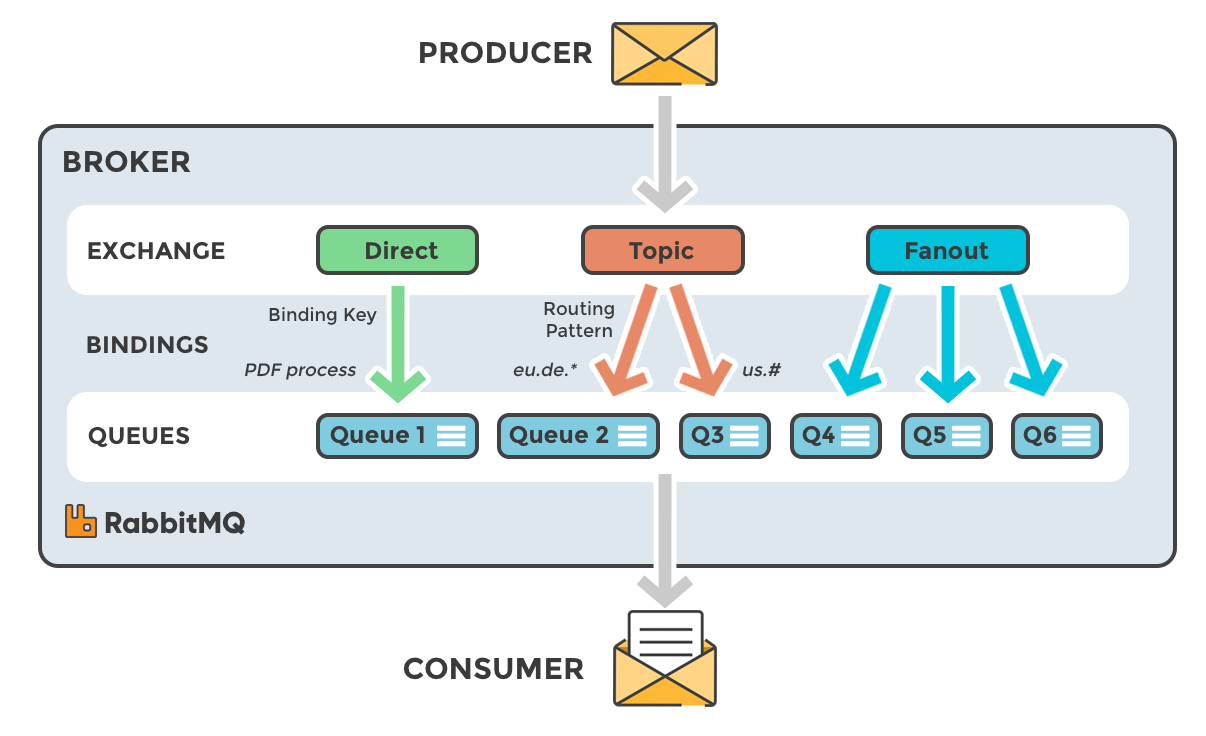
\includegraphics[width=0.45\textwidth]{exchanges-topic-fanout-direct.png}
    \caption{Illustratie van een \emph{message broker}.}\label{fig:broker}
\end{figure}

De applicaties die berichten produceren worden \emph{producers} genoemd en de applicaties die ze consumeren noemen \emph{consumers}. De producers sturen berichten naar een \emph{exchange} op de broker. Op basis van een criterium worden deze berichten dan doorgestuurd naar een wachtrij (\emph{queue}) op de broker, waarop een consumer zich kan abonneren.

Het gebruik van een broker heeft enkele voordelen. Zo is er een ontkoppeling van applicaties; er zijn dus geen directe connecties nodig. Vooral de setup is hierdoor eenvoudiger. 

Ook is er automatisch een vorm van \emph{load balancing}, aangezien meerdere consumers zich kunnen abonneren op een gedeelde wachtrij. Mocht een consumer uitvallen, kunnen de andere consumers dit automatisch opvangen. 

\subsection{Stream-verwerking}\label{ss:stream}
\emph{Stream processing} is een veelgebruikte architectuur voor operaties uit te voeren op een stroom van data. In een gedistribueerde context zijn systemen voor zoals Heron, waarbij operatoren
\subsection{Docker Swarm}\label{ss:swarm}
\subsection{Rapberry Pi}\label{ss:rpi}

\section{Oplossing}

\section{Vergelijking}

\section{Besluit}
\onecolumn

\appendix

\begin{minted}{console}
pi@raspberrypi:~/Documents $ sudo docker service ls
ID                  NAME                MODE                REPLICAS            IMAGE               PORTS
z17loeeu5jp8        eloquent_jepsen     replicated          1/1                 filter:latest       
waucpjaqe1g7        silly_hamilton      replicated          2/2                 transform:latest    
pi@raspberrypi:~/Documents $ sudo docker service scale waucpjaqe1g7=3
waucpjaqe1g7 scaled to 3
overall progress: 3 out of 3 tasks 
1/3: running   [==================================================>] 
2/3: running   [==================================================>] 
3/3: running   [==================================================>] 
verify: Service converged 
pi@raspberrypi:~/Documents $ sudo docker service ls
ID                  NAME                MODE                REPLICAS            IMAGE               PORTS
z17loeeu5jp8        eloquent_jepsen     replicated          1/1                 filter:latest       
waucpjaqe1g7        silly_hamilton      replicated          3/3                 transform:latest    
pi@raspberrypi:~/Documents $ 
\end{minted}

\newpage

% The appendix command is issued once, prior to all appendices, if any.
%\appendix
\end{document}
